\documentclass{beamer}
\mode<presentation>
{
  \usetheme{Berkeley}
  \usecolortheme{dolphin}
  \useinnertheme{rounded}
}

\usepackage[slantfont,boldfont]{xeCJK}
\setCJKmainfont{Songti SC} %mac osx
%\setCJKmainfont{SimSun} windows下使用



\usepackage{fontspec}%字间距控制
\usepackage{tikz}%绘图
\usetikzlibrary{positioning} %on grid
\usetikzlibrary{automata} %style
\usetikzlibrary{shapes,snakes}%各中形状

\usepackage{picinpar}

%%%%%%%%%%%%%%%%%%%
\usepackage[english]{babel}
% or whatever
\usepackage{indentfirst}
\setlength{\parindent}{2em} %首行缩进
\setlength{\parskip}{1em}%段落间距

\usepackage{caption}
\usepackage{multicol}
\usepackage{wrapfig}


\newcommand{\chuhao}{\fontsize{42pt}{\baselineskip}\selectfont}
\newcommand{\xiaochuhao}{\fontsize{36pt}{\baselineskip}\selectfont}
\newcommand{\yihao}{\fontsize{28pt}{\baselineskip}\selectfont}
\newcommand{\erhao}{\fontsize{21pt}{\baselineskip}\selectfont}
\newcommand{\xiaoerhao}{\fontsize{18pt}{\baselineskip}\selectfont}
\newcommand{\sanhao}{\fontsize{15.75pt}{\baselineskip}\selectfont}
\newcommand{\sihao}{\fontsize{14pt}{\baselineskip}\selectfont}
\newcommand{\xiaosihao}{\fontsize{12pt}{\baselineskip}\selectfont}
\newcommand{\wuhao}{\fontsize{10.5pt}{\baselineskip}\selectfont}
\newcommand{\xiaowuhao}{\fontsize{9pt}{\baselineskip}\selectfont}
\newcommand{\liuhao}{\fontsize{7.875pt}{\baselineskip}\selectfont}
\newcommand{\qihao}{\fontsize{5.25pt}{\baselineskip}\selectfont}

\usepackage{times}
\logo{
\includegraphics[height=0.1\textwidth]{figures/tjdx.png}}


\title[图灵奖获得者介绍] % (optional, use only with long paper titles)
{1976年图灵奖获得者}
\subtitle
{Michael O. Rabin,  Dana Steward Scott}

\author% (optional, use only with lots of authors)
{林胤\and 孙渊汇}

\institute
{
  同济大学电子与信息学院
}

\AtBeginSection[]
{
  \begin{frame}<beamer>{内容提纲}
  
  \begin{multicols}{ 2}
      \setlength{\parskip}{0.5em}{\tableofcontents[currentsection,currentsubsection]}
    \end{multicols}
 \end{frame}
}
\begin{document}

\begin{frame}
  \titlepage %封面
\end{frame}
\begin{frame}{内容提纲}
	\begin{multicols}{2}
		\setlength{\parskip}{0.5em}{\tableofcontents}
	\end{multicols}
\end{frame}

\section{简介}
\begin{frame}{1976年的两位图灵奖得主}
	\begin{figure}[htbp]
		\begin{minipage}{0.4\textwidth}
			\centering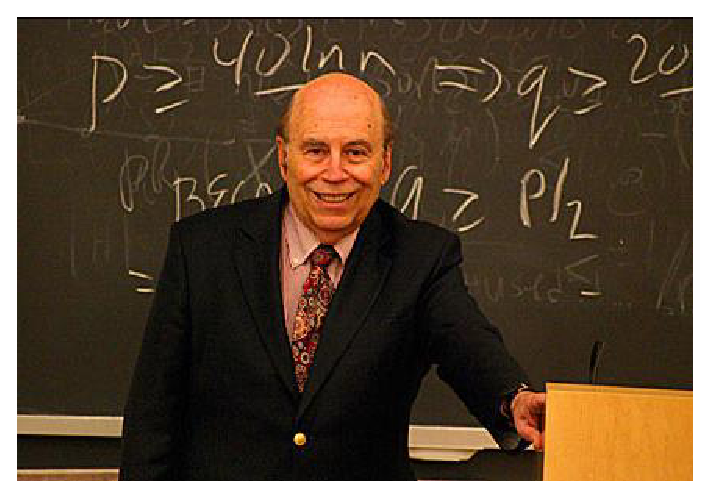
\includegraphics[scale=0.3]{figures/lb2.eps}
			\caption*{Michael O. Rabin}
		\end{minipage}
		\begin{minipage}{0.4\textwidth}
			\centering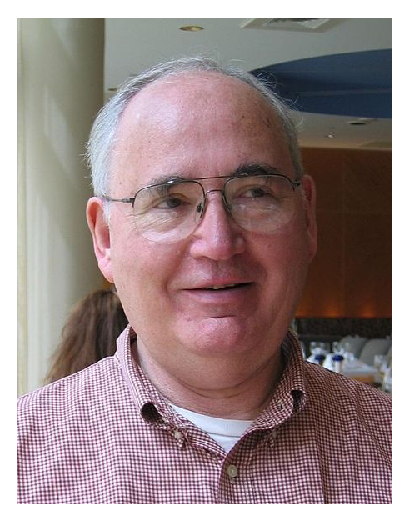
\includegraphics[scale=0.3]{figures/sct.eps}
			\caption*{Dana Steward Scott}
		\end{minipage}
	\end{figure}
\end{frame}

\subsection{迈克尔·拉宾}
\begin{frame}{迈克尔·拉宾}
	\only<1>{
		\begin{figure}[htbp]
			\begin{minipage}[b]{0.3\textwidth}
				\centering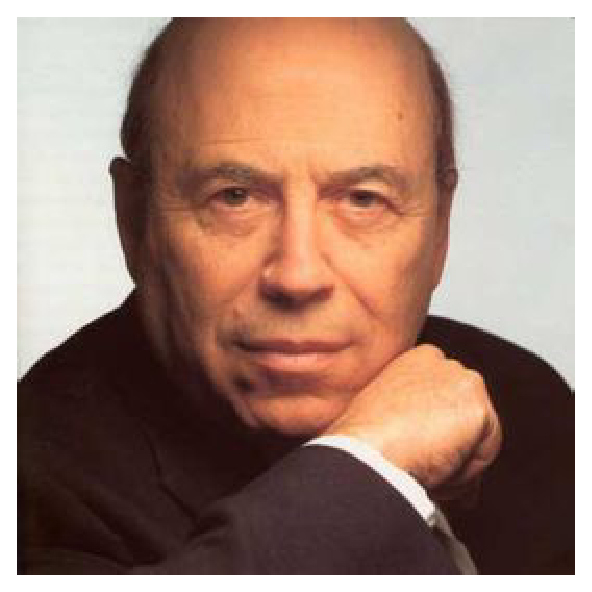
\includegraphics[scale=0.2]{figures/lb.eps}
			\end{minipage}
			\begin{minipage}[b]{0.3\textwidth}
				\centering\includegraphics[scale=0.07]{figures/lb3.eps}
			\end{minipage}
			\begin{minipage}[b]{0.3\textwidth}
				\centering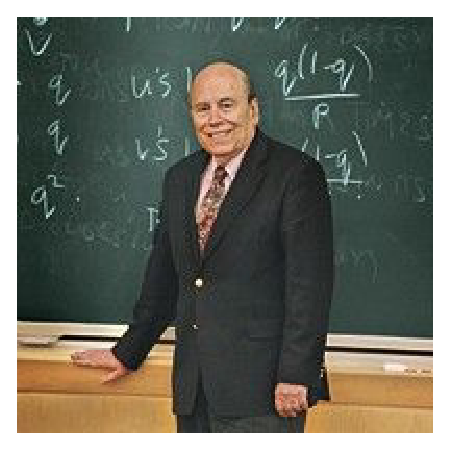
\includegraphics[scale=0.27]{figures/lb4.eps}
			\end{minipage}
			\caption*{\tiny 迈克尔·拉宾}
		\end{figure}
		
		\centering{\wuhao{拉宾现现在就职于哈佛大学\\
				电子邮箱是: \href{mailto:rabin@deas.Harvard.edu}{\textcolor{blue}{\underline{rabin@deas.Harvard.edu}}}\\
				电话:(617) 496-6294
				}}}

	\only<2>{\xiaowuhao{
		\begin{itemize}
			\item 1931年9月1日 出生于德国布雷斯劳(二战后成为波兰弗罗茨瓦夫)
			\item 1953年 获希伯来大学理学硕士(22岁)
			\item 1956年 获普林斯顿大学博士学位(25岁)
			\item 1959年 与达纳斯·斯科特共同发表『有限自动机与其判定性问题』(28岁)
			\item 1975年 发明『米勒-拉宾素数检验』(44岁)
			\item \textcolor{red}{1976年 获得图灵奖,发表『计算复杂性』演讲(45岁)}
			\item 1979年 发明第一个非对称密码系统—拉宾密码系统(48岁)
			\item 1981年 提出『不经意传输』技术(50岁)
			\item 1987年 和查理德·卡普提出字符串搜索『拉宾卡普算法』(56岁)
		\end{itemize}}}
\end{frame}

\subsection{达纳·斯考特}
\begin{frame}{达纳·斯考特}
\only<1>{
	\begin{figure}[htbp]
		\begin{minipage}[b]{0.4\textwidth}
			\centering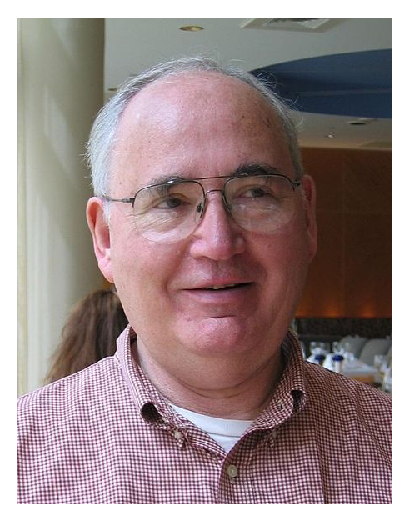
\includegraphics[scale=0.4]{figures/sct.eps}			
		\end{minipage}
		\begin{minipage}[b]{0.4\textwidth}
			\centering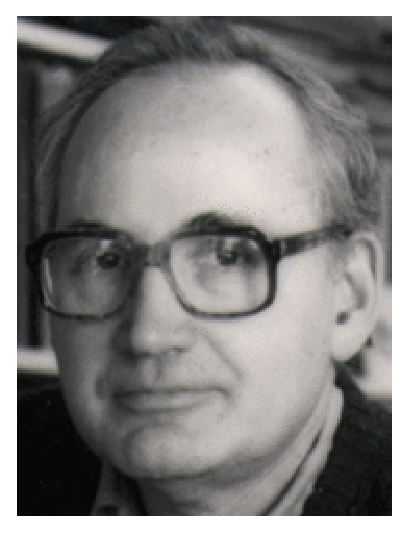
\includegraphics[scale=0.4]{figures/sct2.eps}
		\end{minipage}
	\end{figure}
	
	\centering{\wuhao{斯考特现在就职于卡内基梅隆大学\\
		电子邮箱是:\href{mailto:dana.scott@cs.cmu.edu }{\textcolor{blue}{\underline{dana.scott@cs.cmu.edu}}}\\
		电话:412-268-3881
	}}
	}
\only<2>{\xiaowuhao{\begin{itemize}
		\item 1932年10月11日生于美国加利福尼亚州
		\item 1954年获加州大学伯克利分校学士学位(22岁)
		\item 1958年获普林斯顿大学博士学位(26岁)
		\item 1959年与迈克尔·拉宾共同发表『有限自动机与其判定性问题』(27岁)
		\item 1972年获美国数学协会(AMS)的勒罗伊·斯蒂尔奖(40岁)
		\item \textcolor{red}{1976年获得图灵奖,发表『逻辑与程序设计语言』(44岁)}
		\item 1997年获皇家瑞典皇家科学院颁发的罗尔夫·朔克逻辑和哲学奖(65岁)
		\item 2001年获捷克科学院颁发的博尔扎诺数学优异勋章(69岁)
	\end{itemize}}}
\end{frame}

\tikzset{ state/.style={circle,draw=black}} %定义样式
\tikzset{ term/.style={circle,double,draw=black}}
\tikzset{on/.style={circle,draw=black,fill=red}}

\section{拉宾的故事}
\begin{frame}{拉宾的故事}
\begin{itemize}
\item<1-> 1931年9月1日拉宾出生于德国布雷斯劳(二战后成为波兰弗罗茨瓦夫)的一个拉比家庭,父母是哲学和文学博士
\item<3-> 1935年,由于拉宾的父亲看到了反犹太主义,于是他们居家迁居到巴勒斯坦生活
\item<5-> 之后到了以色列港口城市海法,在一所宗教小学念书
\item<6-> 小时候的拉宾对微生物刚兴趣,一直梦想成为一名微生物学家
\end{itemize}
\begin{figure}[htbp]
	\uncover<2->{\begin{minipage}[b]{0.3\textwidth}\centering
		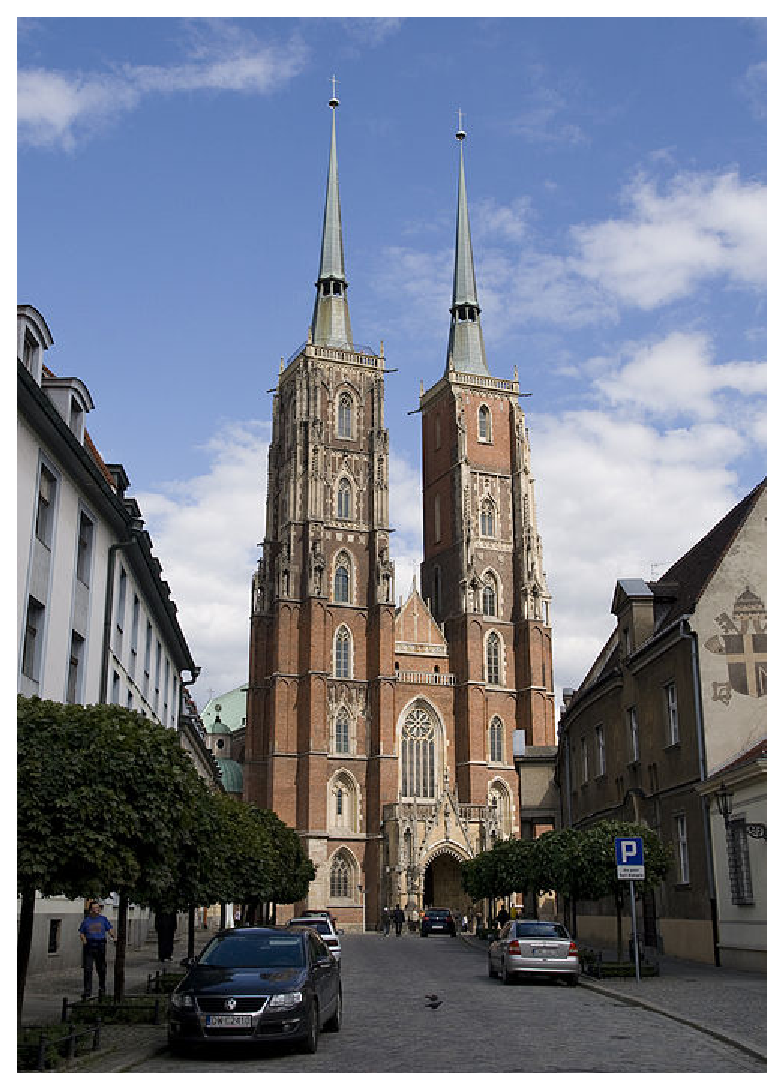
\includegraphics[scale=0.13]{figures/flzwjt.eps}
		\caption*{\tiny 弗罗茨瓦夫大教堂}
	\end{minipage}}
	\uncover<4->{\begin{minipage}[b]{0.3\textwidth}\centering
		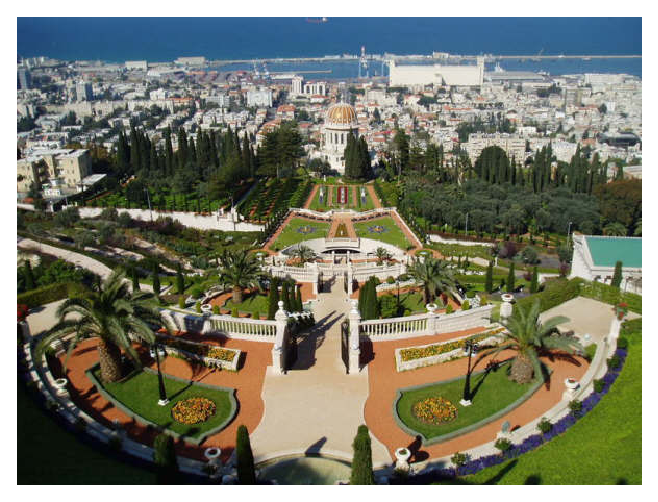
\includegraphics[scale=0.25]{figures/hf.eps}
		\caption*{\tiny 海法中心花园}
	\end{minipage}}
	\uncover<7->{\begin{minipage}[b]{0.3\textwidth}\centering
		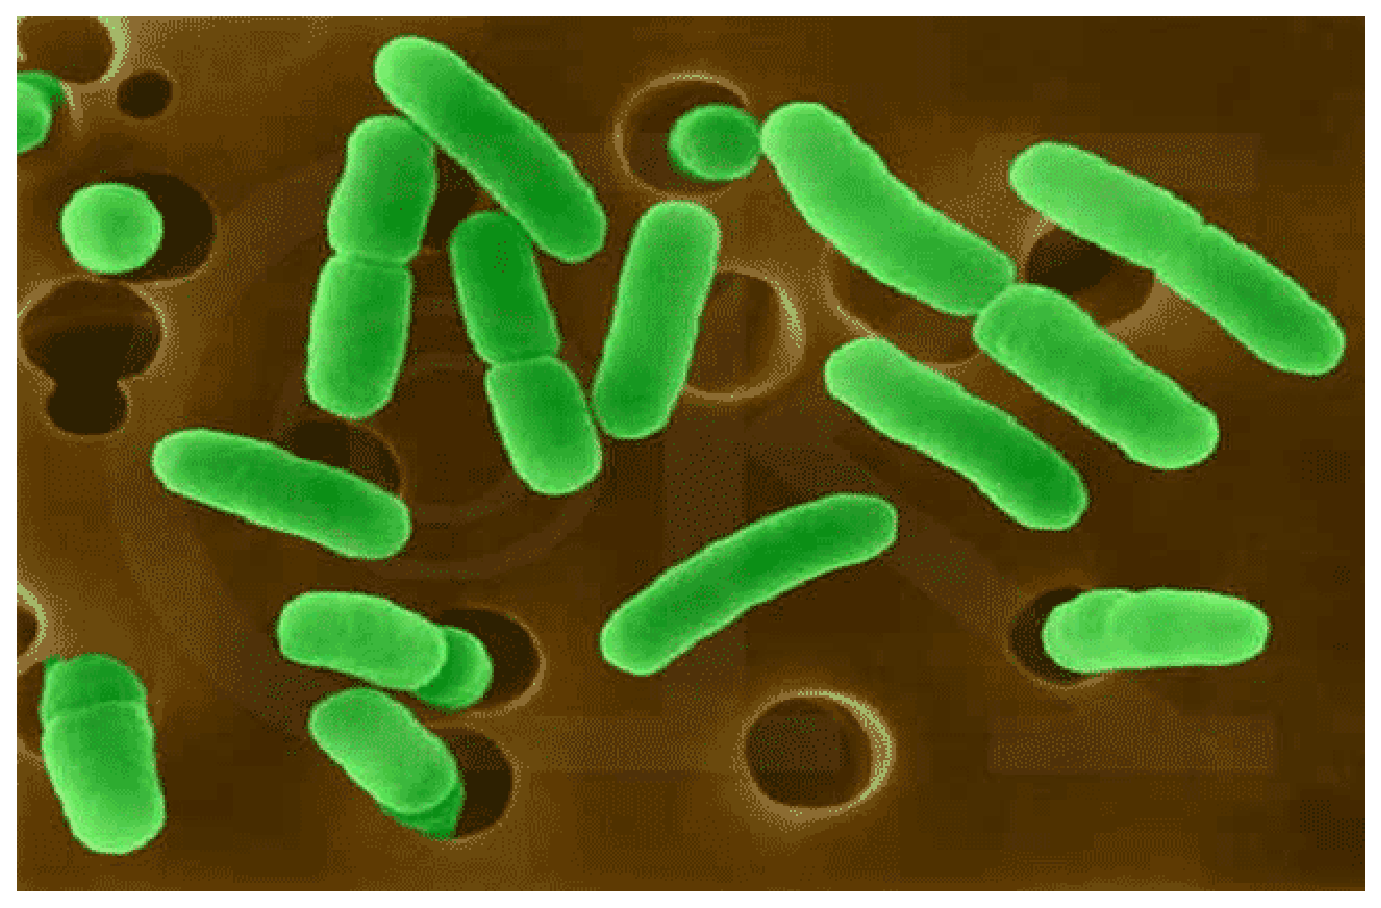
\includegraphics[scale=0.12]{figures/wsw.eps}
		\caption*{\tiny 大肠杆菌}
	\end{minipage}}
\end{figure}
\end{frame}


\subsection{特殊的挑衅}
\begin{frame}{特殊的挑衅}
\begin{figure}
	\begin{minipage}{0.3\textwidth}
		\uncover<2->{\centering\includegraphics[scale=0.05]{figures/jhyb.eps}
		\caption*{\tiny 几何原本中译本}}
	\end{minipage}
	\hfill
	\begin{minipage}{0.65\textwidth}
	\setlength{\parindent}{1.5em}
		\uncover<1->{一天拉宾在教室外面罚站,刚好有两个九年级的学生正那里解欧式几何,拉宾一直站在旁边看。}
		\uncover<2->{恰好他们有个问题解不出来,反过来以此挑衅拉宾。}
		\uncover<3->{偏偏拉宾解出来了,经过证明创建出关于线与圆的真理。}
	\end{minipage}
\end{figure}
	
		
	\uncover<3->{\centering\textcolor{red}{拉宾被其所具有的美所震撼}}
	\vspace{1em}
	
	\uncover<4->{之后拉宾就劝说其父亲将他送去莱利学院学习自然科学知识}
	\end{frame}
	
\subsection{图灵的诱惑}
\begin{frame}{图灵停机}
	\only<1>{英国科学家图灵}\only<2>{提出了一个无法由计算机解决的问题:}
	\only<3>{能否为计算机$X$编程,使其在有限的时间内判断出计算机$Y$上运行的程序是否会停止运行?}%如果计算机Y停止运行,要运行一个程序通知X,则Y又要运行进行检测,显然是一个不可解决问题
	\only<4>{这就是著名的\textbf{\textcolor{red}{图灵停机}}问题。}
	\begin{figure}[htbp]
		\uncover<1->{\begin{minipage}[b]{0.2\textwidth}\centering
			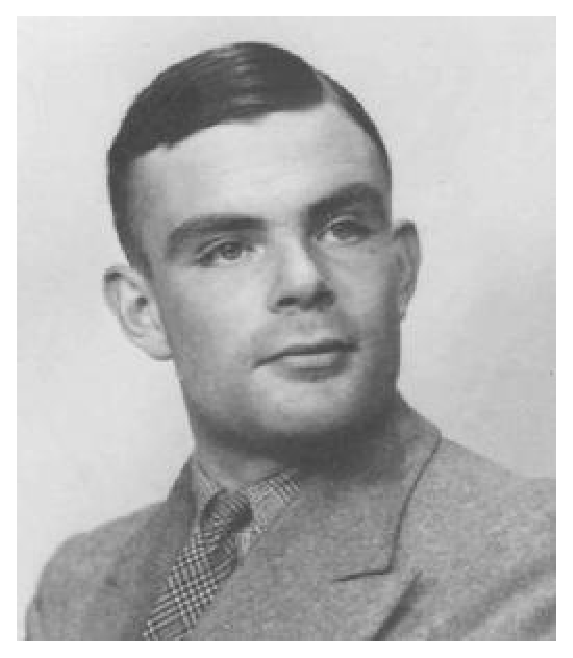
\includegraphics[scale=0.15]{figures/tl.eps}
			\caption*{\tiny 图灵本人}
		\end{minipage}}
		\uncover<4->{\begin{minipage}[b]{0.2\textwidth}\centering
			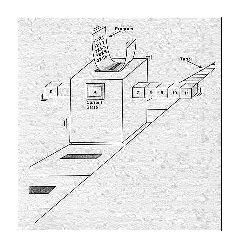
\includegraphics[scale=0.4]{figures/tltj.eps}
			\caption*{\tiny 图灵机}
		\end{minipage}}
		\uncover<5->{\begin{minipage}[b]{0.2\textwidth}\centering
			
\includegraphics[scale=0.2]{figures/bxfny.eps}
			\caption*{\tiny 宾夕法尼亚大学校徽}
		\end{minipage}}
		\uncover<6->{\begin{minipage}[b]{0.2\textwidth}\centering
			
\includegraphics[scale=0.4]{figures/plsd.eps}
			\caption*{\tiny 普林斯顿大学校徽}
		\end{minipage}}
	\end{figure}
	
	\uncover<5->{拉宾对此问题非常痴迷,由于以色列没有计算机,拉宾到了宾夕法尼亚大学攻读数学,}\uncover<6->{然后在普林斯顿大学攻读逻辑学博士。}
\end{frame}

\subsection{完美的合作}
\begin{frame}{注定相遇}
	\begin{itemize}\wuhao{
		\item 拉宾的博士论文讨论了代数群的可计算问题,类似图灵定义了计算上解决与不可解决的界限一样,证明了关于群的某些问题不可计算。
		\pause
		\item 1957年,拉宾还在完成自己的论文,IBM研究院为他和另一位年轻的逻辑学家提供了一份暑期工作,而这个人就是斯科特。
		\pause
		\item 斯考特是逻辑学方面的天才,他们两个人一起研究,提出了一个概念:能够『猜测』的计算机。\pause
		\item 他们的合作是非凡的,往往一个人先提出问题,然后各自回到自己的角落,然后另一个人很快就会给出解决方案。\pause
		\item 大概在三周之内就完成了所有工作,包括在论文中由于篇幅所限未能提及的理论。
		}
	\end{itemize}
\end{frame}

\section{图灵奖内容}
%想办法减少文字
\subsection{DFA与局限性}
\begin{frame}{确定有限自动机(DFA)}
	\only<1>{一个确定有限自动机,对于每一个状态来说,他的下一个状态是确定的。}
	\only<2->{
	\begin{tikzpicture}[shorten >= 1pt, node distance=2cm, on grid, >=stealth]
		\node (start) {start};
		\node[state] (s_0) [right=of start] {0};
		\node[state] (s_1) [right=of s_0] {1};
		\node[state] (s_2) [below=of s_1]{2};
		\node[term] (s_3) [right=of s_1]{3};
		
		\only<2>{\node[on]() at (s_0){0};}
		\only<3>{\node[on]() at (s_1){1};}
		\only<4-5>{\node[on]() at (s_2){2};}
		\only<6>{\node[on]() at (s_3){3};}
		
		\path[->] (start) edge (s_0)
			(s_0) edge node[above]{\textcolor<3>{red}a} (s_1)
				edge node[below left]{b} (s_2)
			(s_1) edge node[above]{b} (s_3)
				edge node[right]{\textcolor<4>{red}a} (s_2)
			(s_2) edge[loop below] node[below] {\textcolor<5>{red}a} ()
			edge node[below right]{\textcolor<6>{red}b} (s_3);
	\end{tikzpicture}
	
	识别串\textcolor<3>{red}a\textcolor<4>{red}a\textcolor<5>{red}a\textcolor<6>{red}b
	}
\end{frame}

\begin{frame}{DFA的局限性}

	\uncover<1->{确定有限自动机每一个状态后面的状态都是确定的,但是现实生活中有很多时候选择并不唯一。}

	\begin{minipage}[h]{0.5\textwidth}
	\setlength{\parindent}{1.5em}
		\liuhao{\textit{\uncover<2->{当我们在餐馆,菜单上有许多菜品,我们可能选择甜点,也可能选择主菜,这不是一个随机过程,但是确实是非确定的。}
		\uncover<3->{当我们选择了某一个种菜品后,我们就进入了另一个状态,结果就是满意或者不满意,也就是接受或者拒绝。}}}
	\end{minipage}
	\hfill
	\begin{minipage}[h]{0.4\textwidth}
		\uncover<2->{\centering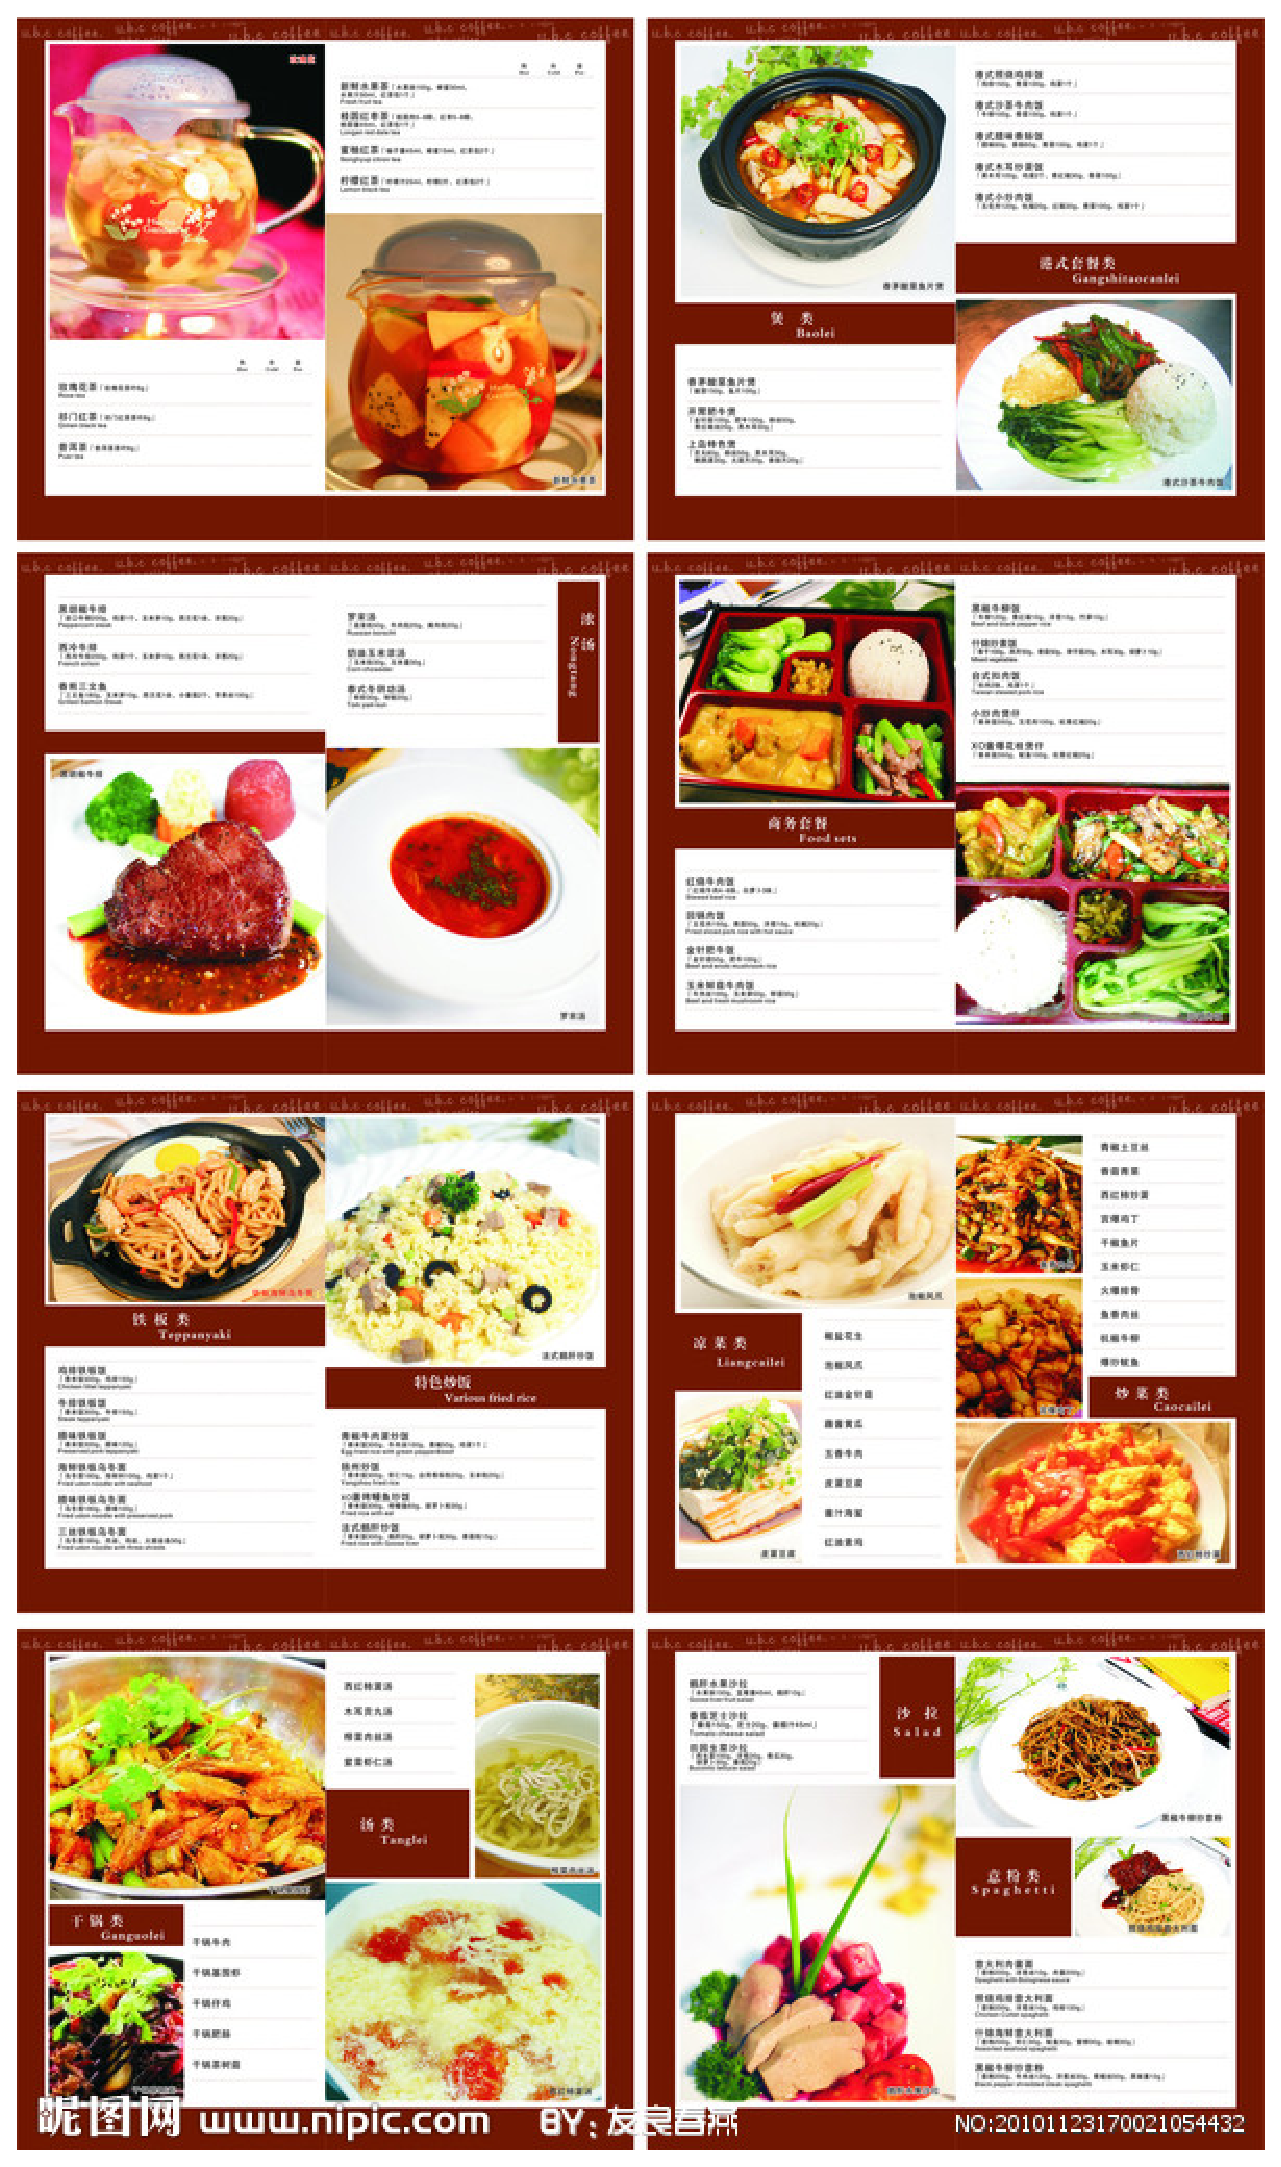
\includegraphics[height=6\baselineskip]{figures/menu.eps}}
	\end{minipage}

	\uncover<4->{不像『确定性』的机器,针对输入只要有任何一种可能达到的『可接受状态』,『非确定性』的机器就会『接受』并运行下去。}

\end{frame}

\begin{frame}{DFA的局限性}
	\begin{itemize}
	\item
	拉宾和斯考特证明,对于有限状态机来说,任何由非确定机解决的问题也可以在确定性机器上解决,并提出了之间的转换方法。
	\item
	非确定有限自动机被证明在语言翻译、文献检索和文字处理程序表达模式搜索的一种绝佳方式。
	\end{itemize}
\end{frame}

\subsection{NFA}
\begin{frame}{非确定有限自动机(NFA)}\wuhao{
\begin{itemize}
	\item<1-> 拉宾和斯考特提出了非确定状态的有限自动机,引入了$\epsilon$
	\item<2-> 非确定状态有限自动机很难用计算机来判别
	\item<3-> 非确定状态有限自动机人很容易写出
	\item<4-> 非确定自动机可以转化为自动机
	\end{itemize}}
\end{frame}

\begin{frame}{非确定有限自动机(NFA)}
使用下面最基本的方法就可以画出任意模式的NFA
	\begin{itemize}
		\only<1->{\item
			$ab$}
		\only<4->{\item
			$a^*$}
		\only<8->{\item
			$a|b$}
	\end{itemize}
	
	\only<2-3>{\centering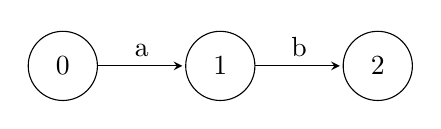
\begin{tikzpicture}[shorten >= 1pt, node distance=2cm, on grid, >=stealth]
		\uncover<2->{\node[state] (s_0)  {0};
		\node[state] (s_1) [right=of s_0] {1};}
		\uncover<3->{\node[state] (s_2) [right=of s_1]{2};}
		\uncover<2->{\path[->](s_0) edge node[above]{a} (s_1);}
		\uncover<3->{\path[->](s_1) edge node[above]{b} (s_2);}
	\end{tikzpicture}}
	\only<5-7>{\centering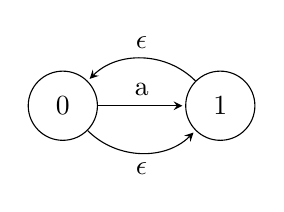
\begin{tikzpicture}[shorten >= 1pt, node distance=2cm, on grid, >=stealth]
		\uncover<5->{\node[state] (s_0)  {0};
		\node[state] (s_1) [right=of s_0] {1};}
		\uncover<5->{\path[->] (s_0) edge node[above]{a}(s_1);}
		\uncover<6->{\path[->] (s_1) edge[bend right=45] node[above]{$\epsilon$} (s_0);}
		\uncover<7->{\path[->] (s_0) edge[bend right=45] node[below]{$\epsilon$} (s_1);}
	\end{tikzpicture}}
	\only<9->{\centering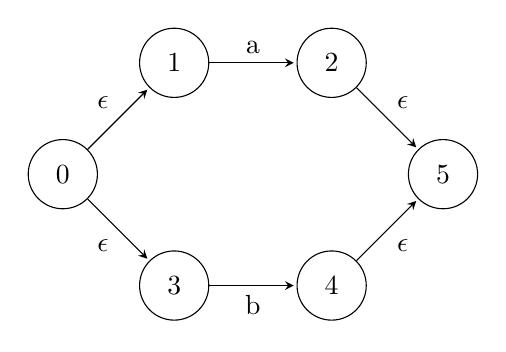
\begin{tikzpicture}[shorten >= 1pt, node distance=2cm, on grid, >=stealth]
		\uncover<10->{\node[state] (s_0) {0};}
		\node[state] (s_1) [above right=of s_0] {1};
		\node[state] (s_2) [right=of s_1] {2};
		\node[state] (s_3) [below right=of s_0] {3};
		\node[state] (s_4) [right=of s_3] {4};
		\uncover<10->{\node[state] (s_5) [below right=of s_2] {5};}
		
		\uncover<10->{\path[->] (s_0) edge node[above left]{$\epsilon$} (s_1)
					edge node[below left]{$\epsilon$} (s_3);}
		\path[->] (s_1) edge node[above]{a} (s_2)
				(s_3) edge node[below]{b} (s_4);
		\uncover<10->{\path[->] (s_2) edge node[above right]{$\epsilon$} (s_5)
				(s_4) edge node[below right]{$\epsilon$} (s_5);}
	\end{tikzpicture}}

\end{frame}

\begin{frame}{NFA试例}
使用刚才的基本模式画出下面模式:$\textcolor<6>{red}{\textcolor<3>{red}{(\textcolor<2>{red}{ab})^*}|\textcolor<5>{red}{(\textcolor<4>{red}{ba})^*}}$
	\begin{figure}\centering
		\begin{tikzpicture}[shorten >= 1pt, node distance=1.5cm, on grid, >=stealth]
			\node(start) {start};
		\uncover<6->{\node[state](s_0) [right=of start]{0};}
		\uncover<2->{\node[state](s_1)[above right =of s_0]{1};
			\node[state](s_2)[right=of s_1]{2};
			\node[state](s_3)[right=of s_2]{3};}
		\uncover<4->{\node[state](s_4)[below right=of s_0]{4};
			\node[state](s_5)[right=of s_4]{5};
			\node[state](s_6)[right=of s_5]{6};}
		\uncover<6->{\node[term](s_7)[below right=of s_3]{7};}
			
		\uncover<2->{\path[->] (s_1) edge node[above]{a} (s_2)
					(s_2) edge node[above]{b} (s_3);}
		\uncover<3->{\path[->] (s_3) edge[bend right=45] node[above]{$\epsilon$} (s_1)
					(s_1) edge[bend right=45] node[above]{$\epsilon$} (s_3);}
		\uncover<4->{\path[->] (s_4) edge node[above]{b} (s_5)
					(s_5) edge node[above]{a} (s_6);}
		\uncover<5->{\path[->] (s_6) edge[bend right=45] node[above]{$\epsilon$} (s_4)
					(s_4) edge[bend right=45] node[above]{$\epsilon$} (s_6);}
		\uncover<6->{\path[->] (s_0) edge node[above left] {$\epsilon$} (s_1)
					(s_0) edge node[below left] {$\epsilon$} (s_4);
			\path[->] (s_3) edge node[above right] {$\epsilon$} (s_7)
					(s_6) edge node[below right] {$\epsilon$} (s_7);
			\path[->] (start) edge (s_0);}
	
			\end{tikzpicture}
		\caption*{\tiny 识别$(ab)^*|(ba)^*$}
	\end{figure}
\end{frame}

\subsection{子集构造法}
\begin{frame}{子集构造法}
	拉宾和斯考特利用集合论的方法提出了任何NFA转换为DFA的算法。\pause
	
	子集构造法就是依次对NFA的状态求闭包运算,闭包中的元素作为一个新状态,然后计算新状态之间的关系。\pause
\end{frame}
\begin{frame}{子集构造法}
\setlength{\parskip}{0em}
\setlength{\lineskip}{0em}
	\qihao{\begin{example}
		\uncover<2->{$T_0 = \epsilon\text{-}closure(0) = \{0,1,3,4,6,7\}$, $move(T_0, a) = \{ 2\}$,$move(T_0, b) = \{5\}$}\\
		\uncover<3->{$T_1 = \epsilon\text{-}closure(2) = \{ 2\}$,$move(T_1, b) = \{3\}$}\\
		\uncover<4->{$T_2 = \epsilon\text{-}closure(5) = \{5\}$, $move(T_2, a) = \{6\}$}\\
		\uncover<5->{$T_3 = \epsilon\text{-}closure(3) = \{1,3,7\}$,$move(T_3,a) = \{2\}$}\\
		\uncover<6->{$T_4 = \epsilon\text{-}closure(6) = \{ 4,6,7\}$, $move(T_4,b) = \{5\}$}\\
		\uncover<7->{$D(T_0, a) = T_1, D(T_0, b) = T_2, D(T_1, b) = T_3$\\
			 $D(T_2, a) = T_4, D(T_3,a) = T_1, D(T_4,b) = T_2$}
		\end{example}}
		\qihao{
		\begin{figure}[htbp]
			\begin{minipage}{0.4\textwidth}
				\begin{tikzpicture}[shorten >= 1pt, node distance=1cm, on grid, >=stealth]
					\node[state](s_0) {0};
					\node[state](s_1)[above right =of s_0]{1};
					\node[state](s_2)[right=of s_1]{2};
					\node[state](s_3)[right=of s_2]{3};
					\node[state](s_4)[below right=of s_0]{4};
					\node[state](s_5)[right=of s_4]{5};
					\node[state](s_6)[right=of s_5]{6};
					\node[term](s_7)[below right=of s_3]{7};
					
					\uncover<2>{\node[on]() at (s_0) {0};}
					\uncover<2,5>{\node[on]() at (s_1) {1};}
					\uncover<3>{\node[on]() at (s_2) {2};}
					\uncover<2,5>{\node[on]() at (s_3) {3};}
					\uncover<2,6>{\node[on]() at (s_4) {4};}
					\uncover<4>{\node[on]() at (s_5) {5};}
					\uncover<2,6>{\node[on]() at (s_6) {6};}
					\uncover<2,5,6>{\node[on]() at (s_7) {7};}
					
					\path[->] (s_1) edge node[above]{\textcolor<2>{red}{a}} (s_2)
							(s_2) edge node[above]{\textcolor<3>{red}{b}} (s_3);
					\path[->] (s_3) edge[bend right=45] node[above]{$\epsilon$} (s_1)
							(s_1) edge[bend right=45] node[above]{$\epsilon$} (s_3);
					\path[->] (s_4) edge node[above]{\textcolor<2>{red}{b}} (s_5)
							(s_5) edge node[above]{\textcolor<4>{red}{a}} (s_6);
					\path[->] (s_6) edge[bend right=45] node[above]{$\epsilon$} (s_4)
							(s_4) edge[bend right=45] node[above]{$\epsilon$} (s_6);
					\path[->] (s_0) edge node[above left] {$\epsilon$} (s_1)
							(s_0) edge node[below left] {$\epsilon$} (s_4);
					\path[->] (s_3) edge node[above right] {$\epsilon$} (s_7)
							(s_6) edge node[below right] {$\epsilon$} (s_7);
				\end{tikzpicture}
			\end{minipage}
			\begin{minipage}{0.4\textwidth}
			\uncover<6->{
				\begin{tikzpicture}[shorten >= 1pt, node distance=1cm, on grid, >=stealth]
					\node(start){start};
					\node[term](t_0) [right=of start]{$T_0$};
					\node[state](t_1)[above right=of t_0] {$T_1$};
					\node[term](t_3)[right=of t_1]{$T_3$};
					\node[state](t_2)[below right=of t_0]{$T_2$};
					\node[term](t_4)[right=of t_2]{$T_4$};
					\uncover<7->{\path[->] (start) edge (t_0)
							(t_0) edge node[above left]{a} (t_1)
							        edge node[below left]{b} (t_2)
							(t_1) edge node[above]{b} (t_3)
							(t_3) edge[bend right=45] node[above]{a} (t_1)
							(t_2) edge node[above]{a}(t_4)
							(t_4) edge[bend left=45] node[below]{b} (t_2);}
				\end{tikzpicture}
			}
			\end{minipage}
		\end{figure}
		}
\end{frame}

\begin{frame}{颁奖词}
因他们的合著论文『有限自动机与其判定性问题』。论文中引入了非确定自动机的概念,被证明是(计算理论科学研究中的)一个非常重要的概念。拉宾和斯科特的这篇经典论文成为了这个领域后续研究的源泉。

\hfill—图灵奖委员会
\end{frame}

\section{计算固有难度}
\subsection{麦卡锡难题}
\begin{frame}{麦肯锡的难题}
\wuhao{
有两个国家处于战争状态。两个国家分别向对方国家派送间谍。间谍完成任务后就返回自己的国家。当他们试图穿越边界时,有可能被自己方的守卫射杀。

所以,他们需要有一套口令机制。假设间谍的素质都很高,能保守秘密。但边界上的守卫经常去当地酒吧聊天—所以不论你告诉他们什么,敌人都能打听出来。

你是否能设计出一套方案,既能让间谍安全的回来,又不让敌人使用从守卫哪里打听到的信息把他们的间谍混进来?}
\end{frame}
\begin{frame}
\wuhao{拉宾采用了一种叫做『单向』函数的算法得出了解决方案。所谓的单项函数,就是一个方向的计算很容易,但是反过来很难。}
	\uncover<2->{\begin{example}
	\uncover<3->{$X = (b_mb_{m-1}b_{m-2}\cdots b_3b_2b_1)_{10}$}
	\uncover<4->{$X^2 = (c_{2m}c_{2m-1}c_{2m-2}\cdots \underbrace{c_{m+m/2}\cdots c_{m-m/2}}_{Y}\cdots c_3c_2c_1)_{10}$}
	\uncover<5->{$Y = (c_{m+m/2}\cdots c_{m-m/2})_{10}$}
	\end{example}}
	
\uncover<6->{\wuhao{通过X计算Y很简单,但是通过Y计算X非常难}}
\end{frame}

\subsection{『世界末日』}
\begin{frame}{固有难度}
\setlength{\parskip}{0em}
	『平方取中』是很难逆向的,那到底有多难?是不是无论采取任何方法,都需要大量的操作?\pause
	
	拉宾进一步地将问题一般化,研究任意给定计算机任务所需的最小工作量,即任务的固有难度。\pause
	
	有些运算是可计算的,但是由于其固有难度非常高,你几乎无法在有限时间内得出结论,所以它的可计算性也就是失去意义了。\pause
	
	\begin{figure}
		\begin{minipage}{0.4\textwidth}\centering
			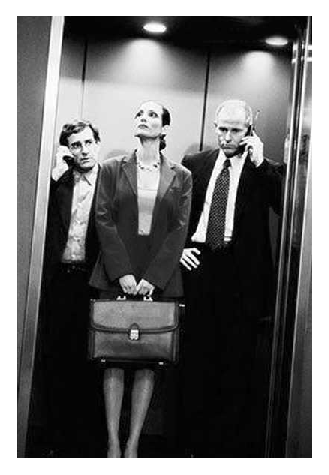
\includegraphics[height=4\baselineskip]{figures/dt.eps}
		\end{minipage}
		\begin{minipage}{0.4\textwidth}\centering
			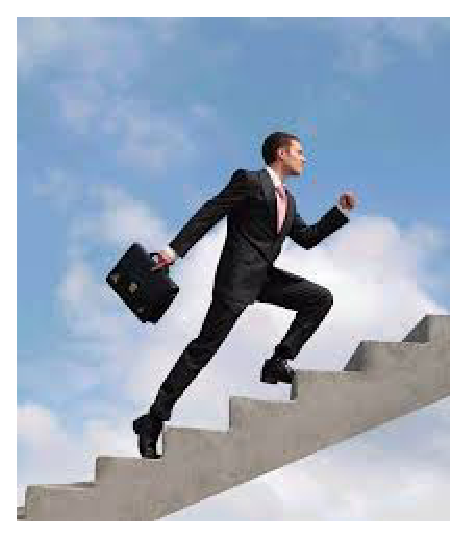
\includegraphics[height=4\baselineskip]{figures/pl.eps}
		\end{minipage}
		\caption*{\tiny 坐电梯和爬楼梯固有难度都是克服重力做功$mgh$}
	\end{figure}
\end{frame}

\begin{frame}{『世界末日』}
	在拉宾那个年代,人工智能界有不少科学家还在执着于编写程序来验证『匹斯伯格系统』的原理。\pause
	
	\textcolor{red}{拉宾宣告了他们的集体失业!}\pause
	
	一个哪怕只有100个符号的系统,即使用1万台每秒一亿次的计算机,也要运行一万亿年。\pause
	
	当拉宾的演讲结束,相关的研究人员都在惊呼这是世界末日,因为他们的实验室可能再也不会得到资助了。
	\begin{figure}
		\begin{minipage}[b]{0.3\textwidth}\centering
			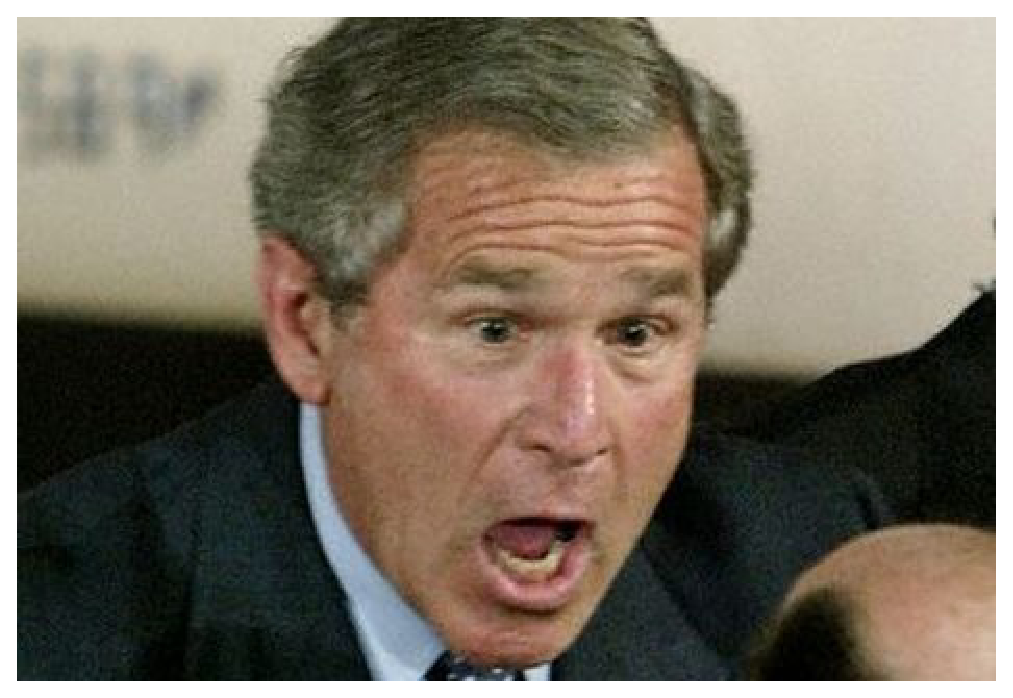
\includegraphics[scale=0.15]{figures/mgd1.eps}
		\end{minipage}
		\begin{minipage}[b]{0.3\textwidth}\centering
			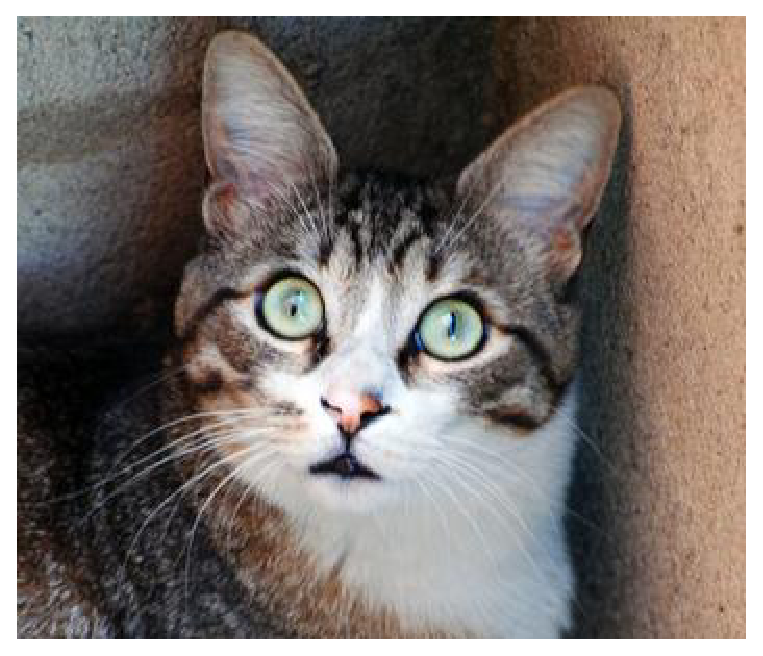
\includegraphics[scale=0.15]{figures/mgd2.eps}
		\end{minipage}
		\begin{minipage}[b]{0.3\textwidth}\centering
			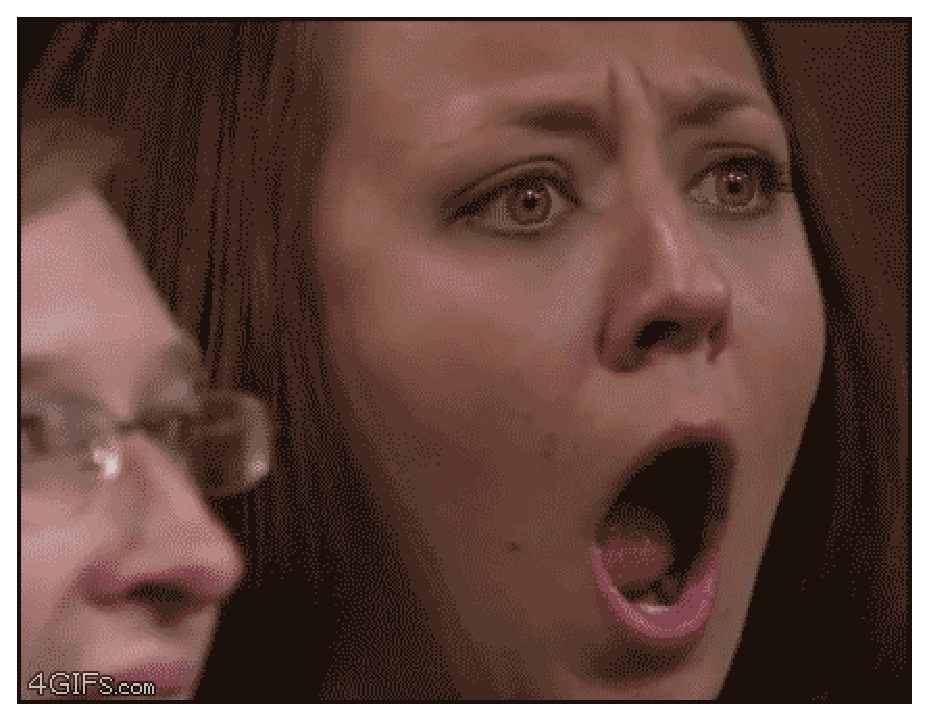
\includegraphics[scale=0.15]{figures/mgd3.eps}
		\end{minipage}
	\end{figure}
\end{frame}

\section{随机性理论}
\begin{frame}{随机性理论}
『在斯德哥尔摩的演讲中,我提出了一个问题:在固有难度这样一个前提下,我们能做什么?』\pause

『我的提议是,应当放弃寻找正确的结果和答案。我们应党适当使用随机性以便更快地得到结果,即便以小小的错误率为代价。』
\end{frame}

\begin{frame}{原始的素数判定算法}
	『素数』一直是数学家很关心的一个问题,而『素数判定算法』也是计算机界一个非常基本的算法。\pause
	
	对于一个数n来说
	\begin{itemize}
		\item 从$\left(1, \sqrt{n} \right]$中依次取数
		\item 逐个验证其是否是$n$的因子
		\item 如果有一个数是$n$的因子,则$n$显然为合数
		\item 否则,我们就宣称n为素数
	\end{itemize}
	
	n的因子就是n传统意义上的见证者。

\end{frame}


\begin{frame}{新式见证者}
	\wuhao{$2^{127}-1$,是一个38位数,要验证它是否为素数,假设计算机每秒钟能运算1亿次除法,那么用当时最好的素数判断算法,也需要\underline{\uncover<2->{\textcolor{red}{93}}}年才能得出结论。}
\end{frame}

\begin{frame}{新式见证者}
	将奇数$n$分解为$2^sd+1$,$d$是一个奇数\pause\\
	对于$a\in\left[2,n-1\right]$\pause\\
	对于$\forall r \in\left[2,s-1\right]$\pause\\
	若$a^d \neq 1$ 且 $a^{2^rd} \neq n-1$\pause\\
	那么$a$就是$n$的见证者。\pause
	\begin{example}
	$27 = 2^1\cdot13+1$ 其旧式见证者\pause\\
	只有$3, 9$\pause\\
	$27$新式的见证者:\pause\\
	只有$1, 26$不是($26^{13} \mod 27 = 26$)\pause\\
	\end{example}

	被证明对于一个很大的数n来说,其新式见证的数量至少是$n$的$3\over4$。
\end{frame}

\begin{frame}{大数素数判断}
	对于一个很大的数n来说
	\begin{itemize}
	\item 从$\left[1, n-1\right]$中随机取150一个数
	\item 逐个验证其是否是『见证者』
	\item 如果有一个数是『见证者』,则n显然为合数
	\item 否则,即150个数中都没有『见证者』,我们就宣称n为素数
	\end{itemize}
\end{frame}

\begin{frame}{错误的概率}
	\uncover<1->{这个结论绝对正确么?}
	\uncover<2->{算法错误的情况是$n$为合数,检验结果数素数。\\}
	\uncover<3->{也就是说必须在150次内每次都避免抽中『见证者』。}
	\uncover<4->{
	\begin{equation*}
		P(error) = \left({1\over4}\right)^{150} \approx  10^{-91}
	\end{equation*}}
	
	\uncover<5->{可能性几乎为0.}
\end{frame}

\begin{frame}{意义}
	\textcolor{blue}{『素数判定理论』的应用}  \\ \pause RSA算法\\
	\textcolor{blue}{『随机性理论』的应用领域} \\ 计算机几何学、分布式计算机、信息检索、密码学、通信学等。
\end{frame}

\section*{Thank You}
\begin{frame}{拉宾的现状}
\begin{figure}
	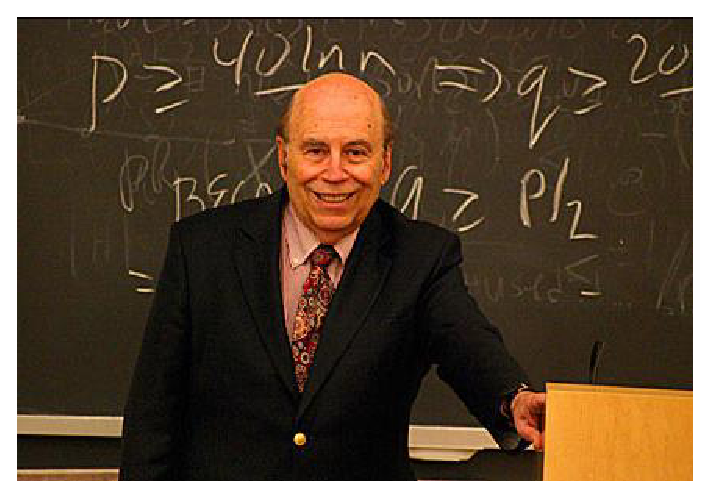
\includegraphics[scale=0.2]{figures/lb2.eps}
\end{figure}
\wuhao{
如今拉宾身为美国哈佛大学计算机科学系教授,同时也是耶路撒冷希伯来大学数学和计算机科学系教授。

他的妻子是以色列司法部国际分布的负责任,一个女儿是律师,另一个女儿是计算机科学家,研究分布式系统和密码学中的随机化理论。

拉宾自己近期的工作是将随机化方法用来(以很高的概率来)确保大型并行计算机的可靠性。}
\end{frame}

\begin{frame}{Thank You}
\liuhao{
林胤
\begin{description}
\item[Blog] \href{http://findingsea.github.io}{\textcolor{blue}{\underline{findingsea.github.io}}}
\item[Github] \href{https://github.com/findingsea}{\textcolor{blue}{\underline{https://github.com/findingsea}}}
\end{description}

孙渊汇
\begin{description}
\item[Blog] \href{http://syhkiller.github.io}{\textcolor{blue}{\underline{syhkiller.github.io}}}
\item[Github] \href{https://github.com/syhkiller}{\textcolor{blue}{\underline{https://github.com/syhkiller}}}
\end{description}

PPT源代码@\href{https://github.com/syhkiller/TuringPPT}{\textcolor{blue}{\underline{https://github.com/syhkiller/TuringPPT}}} \\
forked by \href{https://github.com/findingsea/TuringPPT}{\textcolor{blue}{\underline{https://github.com/findingsea/TuringPPT}}}}
\end{frame}

\end{document}
